\graphicspath{{Chapter_2_-_Notions_of_thermodynamics/Images/}}
\chapter{Notions of thermodynamics}
\quad\, In the introduction, it has been introduced many times the concept and the used of the Brayton cycle. As explained, this concept has been applied for many usages, including electricity production and aircraft propulsion which are the most common and known applications. It has been exposed that from the invention proposed by George Brayton in the end of the 19th century, the technology did really evolve.

Indeed, while the Brayton cycle engine first appears as a  piston engine where the compression, combustion and expansion occurs in the same enclosure, Nowadays 
the process is shared between at least three components (namely the compressor, the turbine and the combustion chamber).

However, what the previous did not cover were the keys notions to understand how theses components behave. Those notions, which will be used during this work, need to be defined and explained to allows to the common person to understand this writing without possessing those knowledge a priory. 
This problematic will be covered by this chapter, which will introduce step-by-step those notions.

\section{Fundamental notions}
\quad\, As mention in the lead-in of this chapter, the first sections of this report will entirely be devoted to the bringing in of the required knowledge for the understanding of the full report.

Starting from very fundamental notions, those will allow to explain more complex concept that will be applied in this work.
\newpage
\subsection{Open/closed system}\label{sect:C2_Sys}
\quad\,  The thermodynamic is a science that "studies the exchange of energy between a system and its environment or surrounding" \cite{thermoApp_1}.

The system is defined as being the area of the space selected for the study. Between the system and the environment lies the boundary. This boundary can either be real or fictitious and, can be static or mobile.

When the system is characterized, it has to be established if it is an open or a closed system.
The open systems are ones where an arbitrary control volume well demarcated in the space is studied. For these systems, matter and energy is exchanged with the surrounding as heat or work. Typical examples are combustion chamber, heat-exchanger, turbomachines, piping,...

On the other hand, the closed systems does not exchange matter with the environment. Indeed, 
for those systems a control mass well delimited in the space is studied. Therefore, the exchange of mass with the environment is prohibited for this category of system. 

\subsection{State functions and variables}\label{sect:C2_State}
\quad\, Let considered a system as defined in the previous section. The state functions are defined as "a property of the system that only depend on its current state". These functions are independent of the past of the system and describe the equilibrium state of the system.

When the state functions can be measured (directly or indirectly), these are called state variables. For example, the pressure $P$, the temperature $T$ or the volume $V$ are state variables.

It can be shown that the equilibrium state of a system can be described by those three variables. Also, among $P$, $T$ and $V$, only two of them are independent. This means that a state relation defined as \textbf{F}($P$, $T$, $V$) = 0.

For the ideal gas, this relation is
\begin{align}
P\cdot V &= m\frac{R}{MM}\cdot T\nonumber\\
P\cdot v &= r\cdot T\label{eq:C2_GP}    
\end{align}
where \textit{m} is the quantity of matter (in kg), $R$ is the universal gas constant (8.314 J/mole/K\footnote{Where K is the degree Kelvin and is scaled as 273.15\degree K = 0\degree C}) and $MM$ is the molar mass (in kg/mole\footnote{Where 1 mole correspond to $\sim 6\cdot 10^{23}$ elementary entities (atoms, molecules,...)}) of the system.
\newpage
\subsection{Energy}\label{sect:C2_Ener}
\quad\, In the subsection \ref{sect:C2_Sys}, the notion of energy has been mentioned without characterizing it before hand. From the first law of thermodynamic, it is stated that the energy cannot be created nor destroyed. Therefore, it can only be converted an can exist into multiple forms (thermal, mechanical, electrical,...)\cite{thermoApp_2}. The unit of the energy is the Joule (J), and the sum of all the energies in a system is called the total energy $E$.

The energy is a state variable. This means that this quantity allows to characterize the state of the system. When considering the energy, its absolute value is not something that is defined. Instead, the energy is always computed as compared with a reference point.

Thus, considering the variation of the total energy from a state \textbf{1} to a state \textbf{2}, it is obtained
\begin{align}
    \Delta E &= \Delta U + \Delta KE + \Delta PE \label{eq:C2_E}\\
    \text{with } \Delta U  &= U_2 - U_1 =  m\cdot(u_2 - u1) \text{: Variation of the internal energy}\nonumber\\
                 \Delta KE &= \frac{1}{2}m\cdot(V^2_2 - V^2_1)\text{: Variation of the kinetic energy}\nonumber\\
                 \Delta PE &= m\cdot g\cdot(z_2 - z_1)\text{: Variation of the potential energy}\nonumber
\end{align} 
where z is the altitude of the system position and U, the internal energy, is the sum of all the "microscopic" energy within the system.

As said in the subsection \ref{sect:C2_Sys}, any system will exchange energy with the surrounding as heat and/or work. The heat is defined as "the form of energy which is exchanged between the system and its environment when there is a gradient of temperature between these two entities". As the heat is always referred as a flux between two bodies, the phenomena is called heat transfer. The heat transfer can be realized by
\begin{itemize}
    \item Conduction: Heat transfer through a non flowing material due to the interaction of "molecular scale energy carriers within the material"\cite{GregoryNellis2015}
    \item Convection: More complex conduction when considering a flowing fluid.
    \item Radiation: The heat is transferred as electromagnetic waves.
\end{itemize}
The heat transfer is denoted $Q$. A system that does not exchange heat with the surrounding is called \textbf{adiabatic}.

Aside the heat transfer, the system also can exchange energy by producing a work. The Work $W$ is "the form of energy exchanged associated to a force applied over a certain distance". The work is exchanged if the force applied on the system creates a displacement of its boundary. The power is defined as the work per unit of time (in Watt or W).

Both the heat and the work are called "path functions" because they are associated to the evolution of a system and not to the state of this system. Thus, these are not thermodynamic variables (like the temperature or the pressure).

\subsubsection{Energy balance}
\quad\, It has been previously mentioned several mechanisms to exchange energy from the system to its environment. Aside from the heat transfer and the work transfer, the energy can also be exchange using mass transfer. Indeed, if the considered system is open, the mass entering and exiting the system will convey energy.

To recall the first principle of thermodynamic, the energy cannot be created or destroyed. Based on the statement, the energy balance of the system is given by the following generic formulation (\ref{eq:C2_EB}).
\begin{equation}
    E_{in} - E_{out} = (Q_{in} - Q_{out}) + (W_{in} - W_{out}) + (E_{mass,in} - E_{mass,out}) = \Delta E_{system} \label{eq:C2_EB}
\end{equation}
with $E_{mass}$ the energy convey by the mass entering/exiting the system.

It is possible to write a temporal formulation (\ref{eq:C2_PB}) of the energy balance named \textbf{power balance}.  
\begin{equation}
    \dot{E}_{in} - \dot{E}_{out} = (\dot{Q}_{in} - \dot{Q}_{out}) + (\dot{W}_{in} - \dot{W}_{out}) + (\dot{E}_{mass,in} - \dot{E}_{mass,out}) = \frac{dE_{system}}{dt} \label{eq:C2_PB}
\end{equation}
where $\frac{dE_{system}}{dt}=0$ when considering a system for which the variation of energy does not vary in the time.

\subsubsection{Energy conservation efficiency}
\quad\, When the system is transferring or converting energy, it is often interesting to quantified the quality of this transfer/conversion. the efficiency is defined to provide this quantification and its definition is the
$\frac{\text{useful product}}{\text{paid consumption}}$. For example, a water electric heater with a efficiency of 90\% is a system such that 90\% of the electrical energy consumed is converted in thermal energy.  

Considering the combustion of a fuel, the combustion efficiency is defined as the ratio
$$ \frac{\dot{Q}}{\dot{m}_{fuel}\cdot HV_{fuel}}$$
where $\dot{m}$  and $HV_{fuel}$ is the mass flow and the heating value of the fuel injected into the combustion chamber.
\section{First principle of thermodynamic}
\quad\, The previous section did introduce many concepts to start analyzing a thermodynamic system submitted to diverse transformations. Among those, the notion of state variables defining the equilibrium state of such system has been defined. this section will introduce the enthalpy and the specific heat based on the first principal of the thermodynamic.

\subsection{Enthalpy}
\quad\, Considering a closed system, the third term of the energy balance given in the relation(\ref{eq:C2_EB}) is nullified. Thus, the variation of the total energy from a state \textbf{1} to a state \textbf{2} is equal to
\begin{equation}
E_{2} - E_{1} = Q_{1-2} - W_{1-2} = (U_2 - U_1) + \frac{1}{2}m\cdot(V^2_2 - V^2_1) + m\cdot g(z_2 - z1)\cite{cogen_1} \label{eq:C2_EBC}
\end{equation}
Let's note that the terms of kinetic and potential energy are often negligible compared to the internal energy.  

The relation \ref{eq:C2_EBC} can be adapted to be applied for the open system by introducing an accumulation term $\Delta E_{cv}$. This correction allows the following reformulation (\ref{eq:C2_EBO}) of the energy balance.
\begin{equation}
Q_{1-2} - W_{1-2} - E_{2} - E_{1} = \Delta E_{cv}\label{eq:C2_EBO}
\end{equation}

\begin{figure}[h]
\centering
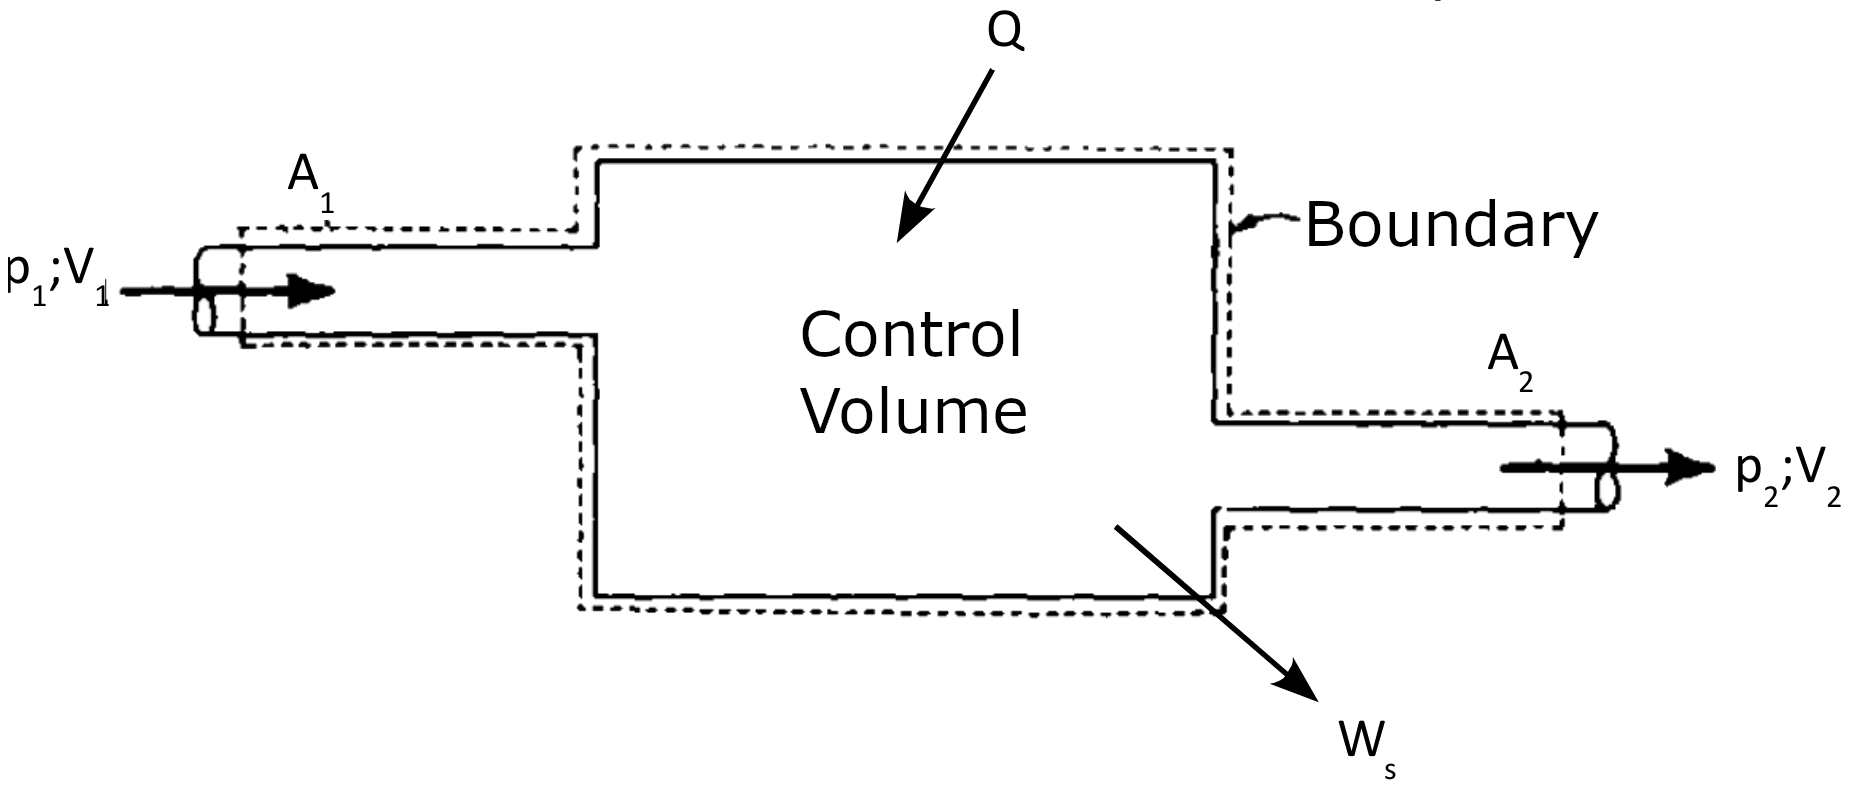
\includegraphics[width=0.8\textwidth]{control_volume.png}
\caption{System control volume}
\label{fig:C2_VC}
\end{figure}

The Figure \ref{fig:C2_VC} depicts a open system with an entry and exit area $A_1$ and $A_2$ respectively. Posing that the work $W$ is equal to 
\begin{equation}
W = P_2\cdot A_2\cdot V_2\Delta t - P_1\cdot A_1\cdot V_1\Delta t + W_s
\end{equation}      
where $P_1$ (resp. $P_2$) and $V_1$ (resp. $V_2$) are the pressure and the velocity at \textbf{1} (resp. \textbf{2}).

By neglecting the variation of the kinetic and potential energy, the energy balance is after some mathematical operations as given in the relation \ref{eq:C2_EBH}
\begin{equation}
q - w_s = u_2 +P_2\cdot v_2 - u_1 - P_1\cdot v_1 = h_2 - h_1\label{eq:C2_EBH}
\end{equation}
where $q$, $w_s$ and $h$ are the specific work, heat and \textbf{enthalpy} (in J/kg).  
For the case of an ideal gas, the enthalpy and the internal energy only depend on the temperature $T$. Indeed, taking the equation (\ref{eq:C2_GP}), the relation (\ref{eq:C2_h}) can easily be deduced.
\begin{equation}
h = u(T) + Pv = u(T) + rT \label{eq:C2_h}
\end{equation}
\subsection{Specific heat}
\quad\, The previous subsection was meant to define the enthalpy. This state variable is used in place of the internal energy when dealing with open system.\\

An other quantity that is useful for system study is the \textbf{specific heat}. This state variable is defined as the required energy to increase of 1\degree C the temperature of 1kg of a substance. 
 
The required heat to produce this effect depends on the ways the transformation takes place. 
If it is done under constant volume constraint, it is called specific heat at constant volume and denoted $c_v$. 

If the transformation is performed at constant pressure, the symbol associated to the specific heat is $c_p$.
It is worth to note that the specific heat at constant pressure is always higher than the $c_v$. When performing the transformation a constant pressure, the gas "expands against the external pressure. This means that the gas does work"\cite{Ashutoshvashisht202017}. This is the reason why the supplied heat has to be greater than for the transformation at constant volume. 

It had been shown that for an ideal gas, the variation of the internal energy can be linked to the specific heat at constant volume as written in the relation (\ref{eq:C2_UC}).
\begin{equation}
du = c_vdT \rightarrow u_2 - u_1 = \int_{T_1}^{T_2} c_vdT\label{eq:C2_UC}
\end{equation} 
Similarly, the variation of the enthalpy can be expressed using the specific at constant pressure.

\begin{equation}
dh = c_pdT \rightarrow h_2 - h_1 = \int_{T_1}^{T_2} c_pdT\label{eq:C2_UP}
\end{equation} 

These two relations, with the equality (\ref{eq:C2_h}), provide the required tools to express the gas constant $r$ as a function of the temperature only. 
\begin{equation}
r = c_p - c_v \label{eq:C2_r}
\end{equation}

Aside the gas constant, the ratio of the specific heat $\lambda$ (\ref{eq:C2_lbd}) is also a useful variable to be computed.
\begin{equation}
\lambda = \frac{c_p}{c_v} \label{eq:C2_lbd}
\end{equation}

As shown in this section, the first principle of termodynamic provid